\lecture{10}{26. Februar 2025}{Failure Mechanisms, Pt. 2: Fatigue and Creep}

Use the cyclic stresses represented by the graph below to answer the following questions.
\begin{figure} [ht]
  \centering
  \caption{}
  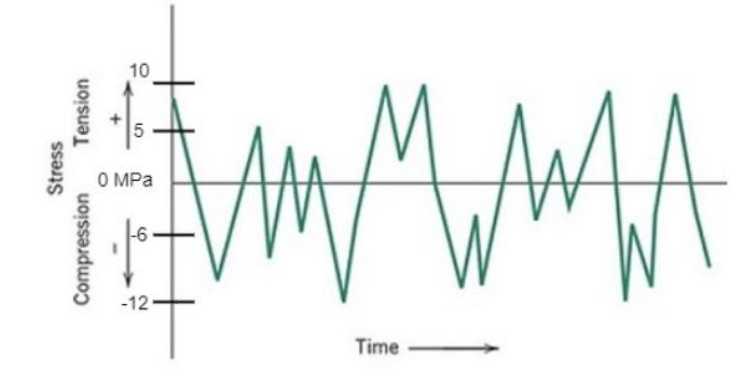
\includegraphics[width=0.5\linewidth]{./figures/f10_1.png}
  \label{fig:f10_1}
\end{figure}

\paragraph{1)} The mean stress, $\sigma_m$ is
\bigbreak
The mean stress can be calculated as
\[ 
\sigma_m = \frac{-12 + 10}{2} = -1
.\]

\paragraph{2)} The range of stress, $\sigma_r$ is
\bigbreak
The range of stress is
\[ 
\sigma_r = 10 - (-12) = 22
.\]


\paragraph{3)} The stress amplitude, $\sigma_a$ is
\bigbreak
The stress amplitude is
\[ 
\sigma_a = \frac{10 - (-12)}{2} = 11
.\]


\paragraph{4)} The stress ratio, $R$ is
\bigbreak
The stress ratio is
\[ 
R = \frac{-12}{10} = -\frac{6}{5}
.\]



\exercise{8.D3} For an 18--8 $Mo$ stainless steel (\textbf{\autoref{fig:f10_2}}), predict the time to rupture for a component that is subjected to a stress of \qty{100}{MPa} at \qty{600}{\celsius} (\qty{873}{K}).
\begin{figure} [ht]
  \centering
  \caption{}
  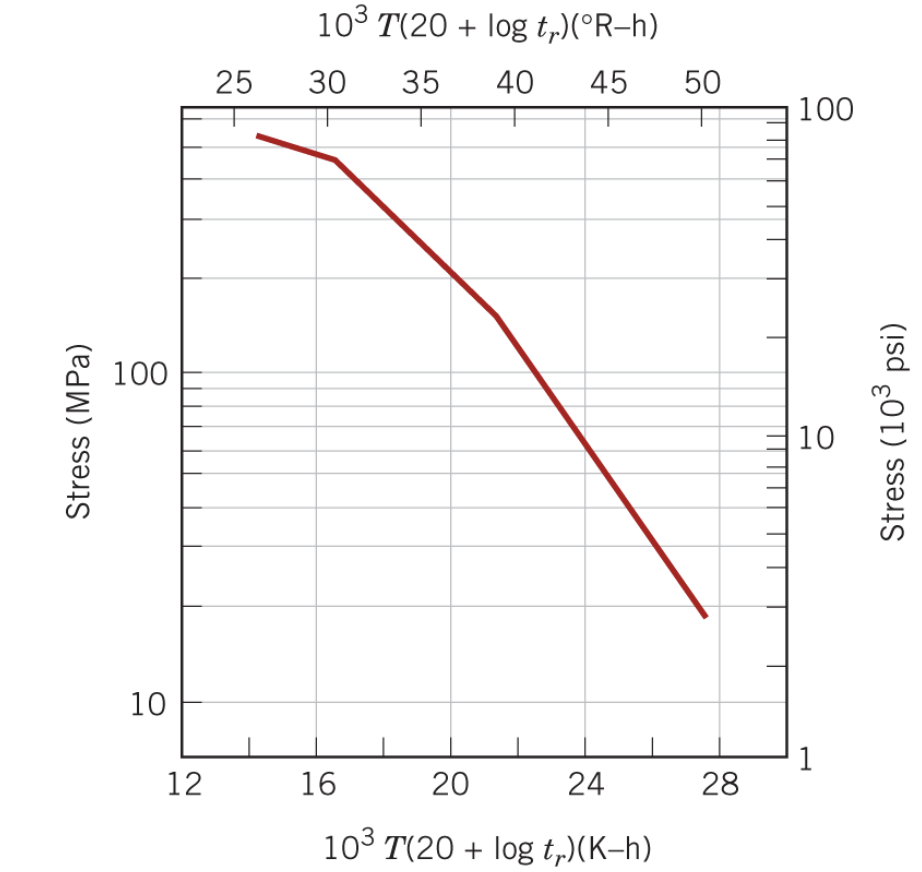
\includegraphics[width=0.5\linewidth]{./figures/f10_2.png}
  \label{fig:f10_2}
\end{figure}
\bigbreak
From the given figure we can determine the Larsson-Miller parameter at \qty{100}{MPa} to be about \num{22,6e3} for $T$ in \unit{K} and time in \unit{hr}. Therefore
\[ 
\num{22,6e3} = T \left( 20 + \log t_r \right) = 873(20 + \log t_r)
.\]
Which leads to
\begin{align*}
  \num{25,89} &= 20 + \log t_r \\
  \num{5,89}  &= \log t_r \\
  t_r &= 10^{\num{5,89}} = \qty{89}{yr} 
.\end{align*}
